\documentclass{beamercours}

\title{Deriving Geodesics on a 3D Mesh from the Heat Equation}
\author{Matthieu Boyer}
\def\mF{\mathcal{F}}
\def\mV{\mathcal{V}}
\DeclareMathOperator{\id}{\mathrm{id}}

\begin{document}
\maketitle

\section{Introduction}
\begin{frame}
	\frametitle{Geodesics}
	\begin{figure}[h]
	\centering
	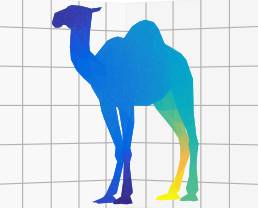
\includegraphics{Figures/camel_geodesics.png}
	\caption{An application of our method: a dromedary stepping on a hot rock}
	\label{camel}
\end{figure}
\end{frame}

\begin{frame}[allowframebreaks]
	\frametitle{Varadhan's Formula}
	Remember the Heat Equation:
	\begin{equation}
		\tag{Heat}
		\boxed{\Delta H = \frac{\partial}{\partial t} H}
	\end{equation}
	We will use it to compute the geodesics, following \cite{heatgeodesics}.
	\framebreak
	\begin{théorème}{Varadhan's Formula \cite{varadhan}}{varadhan}
		If $(M, g)$ is a complete Riemannian manifold, and $k_{t, x}(y)$ is the associated heat kernel, converging to $\delta_{x}(y)$ at small times, then:
		\begin{equation}
			\tag{VF}
			\boxed{-4t \log k_{t, x}(y) \xrightarrow[t \to 0]{} d\left( x, y \right)^{2}}
			\label{varadhanformula}
		\end{equation}
		where $d$ is the distance function on the manifolds.
	\end{théorème}
\end{frame}

\section{Related Work and Applications}
\begin{frame}[allowframebreaks]
	\frametitle{Related Work}
	The most widely used method is solving:
	\begin{equation}
		\norm{\nabla \phi} = 1 \text{ subject to boundary conditions } \phi_{\mid \gamma} = 0
	\end{equation}
	but it needs $\O\left( n\log n \right)$ and $\O(n)$ time per step in the Gauss-Seidel algorithm and loses information.
	\framebreak

	Another method based on Schrödinger's equation has been proposed in \cite{schrod} which ressembles ours, but with more limitations and a need for arbitrary precision on $\hbar$ needed:
	\begin{equation}
		H\psi\left( x \right) = E\psi\left( x \right) \text{ where } H = -\frac{\hbar^{2}}{2m}\Delta + V(x)
	\end{equation}
\end{frame}

\begin{frame}
	\frametitle{Applications}
	\begin{itemize}
		\item Image Analysis: \cite{geodesicmetricuse} by Lantuejoul and Beucher
		\item Heuristically-driven Propagation: \cite{Peyré2009}
		\item Solidworks
	\end{itemize}
\end{frame}

\section{The Method}
\begin{frame}[fragile]
	\frametitle{The Algorithm}
	\begin{algorithm}[H]
		\caption{The Heat Method}
		\label{heatmethod}
		\begin{enumerate}
			\item Integrate $\dot{u} = \Delta u$ for some fixed time $t$.
			\item Evaluate the vector field $X = \frac{-\nabla u}{\norm{\nabla u}}$.
			\item Solve the Poisson equation $\Delta \phi = \nabla \cdot X$.
		\end{enumerate}
	\end{algorithm}
	Initial conditions allow for a single source point or any piecewise submanifold.
\end{frame}

\begin{frame}[allowframebreaks]
	\frametitle{Discretizing Time}
	We use a single backward Euler step:
	\begin{equation}
		\left( \id - t\Delta \right)u_{t} = u_{0}
	\end{equation}
	our problem is then solving:
	\begin{equation}
	\tag{BP}
	\begin{array}{rcl}
		\left( \id - t\Delta \right)v_{t} = 0 & \rm on & M\setminus \{x\}\\
		v_{t} = 1 & \rm on & x
	\end{array}
	\label{boundaryproblem}
	\end{equation}
	\framebreak

	The correction of the algorithm comes from the proof of Theorem \ref{thm:varadhan} in \cite{varadhan}:
	\begin{equation}
		\tag{$\delta t$}
		-\frac{\sqrt{t}}{2}\log v_{t} \underset{t \to 0}{=} \phi
		\label{discretetime}
	\end{equation}
\end{frame}

\begin{frame}[allowframebreaks]
	\frametitle{Discretizing Space}
	We only need a gradient $\nabla$, divergence $\nabla \cdot$ and laplacian $\Delta$.
	We consider a triangulation $\left(\mV, \mF \subseteq \mV^{3}\right)$.
	\framebreak

	The gradient of $u$ in a given triangle $f$ is:
	\begin{equation}
		\nabla_{f} u = \frac{1}{2A_{f}}\sum_{i \in f} u_{i}\left( N \land e_{j_{i}} \right)
	\end{equation}
	and, as a matrix of size $3\abs{\mF} \times \abs{\mV}$:
	\begin{equation}
		\begin{aligned}
			\left(\tilde{\nabla}\right)_{i, j} =& \left( \vec{Je_{j_{i}}} \right)_{1}\\
			\left(\tilde{\nabla}\right)_{i + \abs{\mF}, j} =& \left( \vec{Je_{j_{i}}} \right)_{2}\\
			\left(\tilde{\nabla}\right)_{i + 2\abs{\mF}, j} =& \left( \vec{Je_{j_{i}}} \right)_{3}
		\end{aligned}
	\end{equation}

	Then, we can compute the divergence operator's matrix as the transpose of the gradient for the face area dot product:
	\begin{equation}
		\nabla\cdot = \nabla^{T}A
	\end{equation}
	where $A$ is defined as previously as a $3\abs{\mF}$ diagonal matrix containing the areas of the faces.
	\framebreak

	Finally:
	\begin{equation}
		\Delta = \nabla \cdot \nabla = \nabla^{T}A\nabla
	\end{equation}
	which is coherent with:
	\begin{equation}
		\left( Lu \right)_{i} = \frac{1}{2VA_{i}}\sum_{j \in \mathcal{N}\left( i \right)}\left( \cot\alpha_{i, j} + \cot\beta_{i, j} \right)\left( u_{j} - u_{i} \right)
	\end{equation}
	We will call $L_{C}$ the sum part of this operator.
	Then, retrieving our distance function amounts to solving: $\left(VA - tL_{C}\right)u = u_{0}$ and then $L_{C}\phi = \nabla\cdot \left( \frac{-\nabla u}{\norm{\nabla u}} \right)$.
\end{frame}

\begin{frame}[allowframebreaks]
	\frametitle{Time Step}
	\begin{théorème}{Graph Distance}{combi}
	Let $G = \left( V, E \right)$ be the graph induced by any real symmetric matrix $A$, and consider:
	\begin{equation*}
		\left( \Id - t A \right)u_{t} = \delta
	\end{equation*}
	where $\delta$ is a Kronecker delta at a source vertex $u \in V$ and $t > 0$. Then:
	\begin{equation*}
		\boxed{\phi_{G} = \lim_{t \to 0} \frac{\log u_{t}}{\log t}}
	\end{equation*}
	\end{théorème}
	\framebreak

	For $t < \frac{1}{\sigma}$:
	\begin{equation*}
		u_{t} = \sum_{k = 0}^{\infty} t^{k}A^{k}\delta
	\end{equation*}
	Let $v \in V$ be $n$ edges away from $u$ and consider $r_{t} = \abs{R_{v}}/\abs{s_{v}}$ where:
	\begin{equation*}
		s_{v} = \left( t^{n}A^{n}\delta \right)_{v} \neq 0, \qquad R_{v} = \left( \sum_{k = n + 1}^{\infty}t^{k}A^{k}\delta \right)_{v}
	\end{equation*}
	\framebreak

	Since:
	\begin{equation*}
		\abs{s} \leq \sum_{k \geq n + 1} t^{k}\norm{A^{k}\delta} \leq \sum_{k \geq n + 1}t^{k}\sigma^{k}
	\end{equation*}
	and thus:
	\begin{equation*}
		r_{t} \leq \frac{t^{n + 1}\sigma^{n + 1}\sum_{k = 0}^{+\infty}t^{k}\sigma^{k}}{t^{n}\left( a^{n}\delta \right)_{v}} = c\frac{t}{1 - t\sigma}
	\end{equation*}
	Finally:
	\begin{equation*}
		\log s_{0} = n\log t + \log \left( A^{n}\delta \right)_{v}
	\end{equation*}
\end{frame}

\section{Implementation}
\begin{frame}
	\frametitle{Complexity}
	Our time complexity is:
	\begin{equation*}
		\O\left( \abs{\mF}^{2} \right)
	\end{equation*}
	and our space complexity is:
	\begin{equation*}
		\O\left( \abs{\mF}\abs{\mV} \right)
	\end{equation*}
	when taking our matrix representation as sparse as possible, while not increasing our time complexity too much.
\end{frame}

\begin{frame}[allowframebreaks]
	\frametitle{Benchmarks}
	We used the following mesh for the $\left[ 0, 1 \right] \times \left[ 0, 1 \right] \times 0$ square embedded in the $3$-dimensional euclidean space:
	\begin{align*}
		\mV = \left\{ \left( k\epsilon, k'\epsilon \right) \ \middle| \ 0 \leq k, k' \leq \frac{1}{\varepsilon} \right\}\\
		\mF = \left\{ \left( i, i + 1, i + n \right), \left( i, i + n, i + n -1 \right) \ \middle| \ i \leq \frac{1}{\epsilon^{2}} \right\} \cap \mV^{3}
	\end{align*}
	\framebreak

	Here, the average distance between two connected points is thus given by:
	\begin{equation*}
		h = \frac{4}{6}\epsilon + \frac{2}{6}\sqrt{2}\epsilon = \frac{2 + \sqrt{2}}{3}\epsilon \simeq 1.14 \times \epsilon
	\end{equation*}
	and thus $t = 1.3\epsilon^{2}$.

\end{frame}

\begin{frame}[allowframebreaks]
	\frametitle{Results in time Complexity}
	\begin{figure}[h]
		\centering
		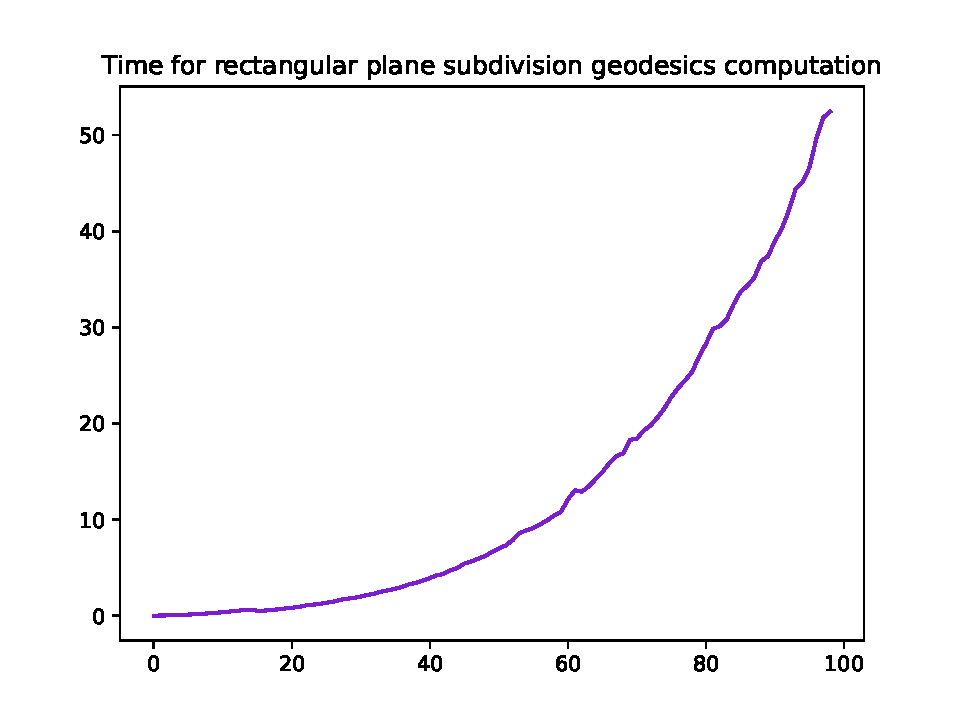
\includegraphics[scale=.4]{Figures/tim_comp_planes_i<=100}
		\caption{Computation times for evenly spaced triangular mesh of step $1/i$ on the unit square.}
		\label{computationtime}
	\end{figure}
	\framebreak


	\begin{figure}[h]
		\centering
		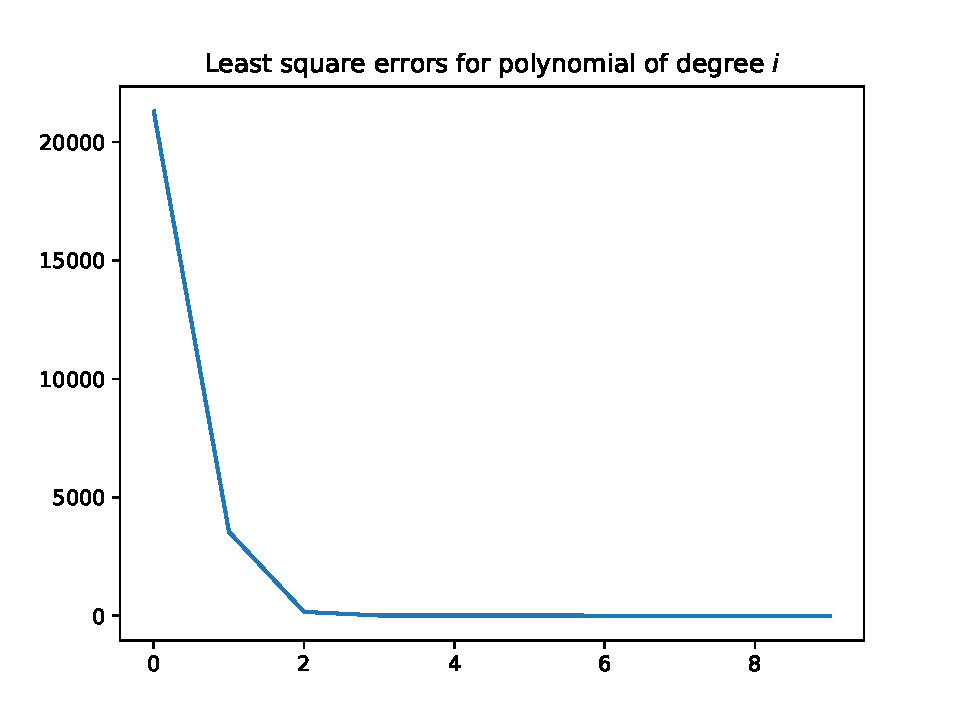
\includegraphics[scale=.4]{Figures/polyfiterrors}
		\caption{Errors of fit for polynomials of degree up to $10$ for the computation time presented before, using the $\ell^{2}$ norm.}
		\label{polyfiterrors}
	\end{figure}
\end{frame}

\begin{frame}[allowframebreaks]
	\frametitle{Theoretical Accuracy}
	Let us take our plane mesh defined by $\epsilon$. The geodesic distance to $0$ can be directly computed:
	\begin{equation*}
		d\left( x \right) = \norm{x} \text{ and on indices } d_{\epsilon}\left( i \right) = \epsilon\sqrt{\left( i \mod \frac{1}{\epsilon} \right)^{2} + \left( i // \frac{1}{\epsilon} \right)^{2}}
	\end{equation*}
	\framebreak

	\begin{figure}[H]
		\centering
		\resizebox{.5\textwidth}{.5\textwidth}{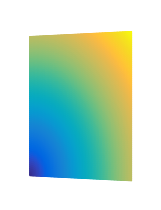
\includegraphics{Figures/plane_geodesics}}
		\caption{Illustration of the geodesic distance from $0$ on the evenly spaced mesh of step $1/70$ on the plane}
	\end{figure}
	\framebreak

	Then in theory:
	\begin{equation*}
		d\left( i \right) - \epsilon\phi\left( i \right) \leq \frac{\epsilon}{2} \left(\left( i \mod \frac{1}{\epsilon} \right) + \left(i // \frac{1}{\epsilon} \right) \right)
	\end{equation*}
\end{frame}

\begin{frame}
	\frametitle{Practical difference to theoretical difference}
	\begin{figure}[H]
		\centering
		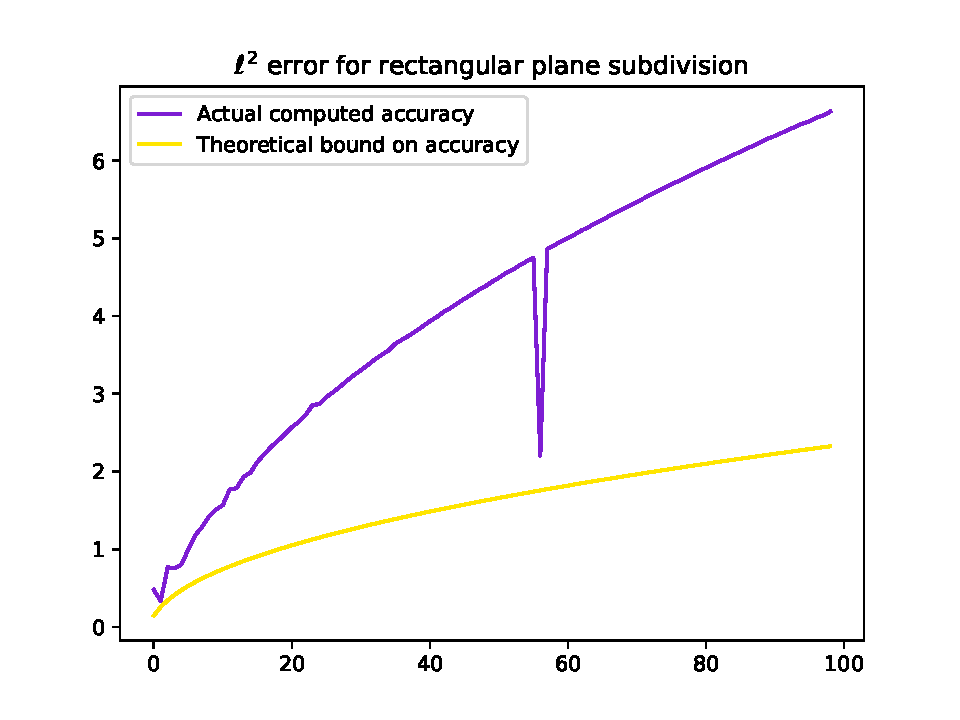
\includegraphics[scale=.4]{Figures/compare_err_comp_planes_i<=100}
		\caption{Theoretical bound on accuracy of the heat methods for regular meshes for the plane of step $1/i$}
	\label{planediff}
\end{figure}
\end{frame}


\section{References}
\begin{frame}[t, allowframebreaks]
	\frametitle{References}
	\bibliographystyle{alpha}
	\bibliography{report}
\end{frame}

\end{document}
